%%%%%%%%%%%%%%%%
% Ph.D. thesis %
%%%%%%%%%%%%%%%%
%\documentclass[11pt,openright,twoside,letterpaper,onecolumn]{report} %% USE THIS FOR DOUBLE SIDED
\documentclass[11pt,openright,oneside,letterpaper,onecolumn]{report}  %% USE THIS FOR SINGLE SIDED
\newcommand{\thesistitle}{New Methods in Sampling in Molecular Mechanics Simulations and and Improved Algorithm for Calculating Energy Contribution of Implicit Solvent Models}
\newcommand{\thesisauthor}{Joseph Bylund}
\newcommand{\thesisyear}{2013}

%%%
%%% Packages
%%%
\usepackage[dvips]{epsfig}
\usepackage{amsmath}
\usepackage{named}
\usepackage{fancyhdr}
\usepackage{afterpage}

%
% We use the hyperref package and customize it for optimal PDF 
%
%\usepackage[dvipdfm,pdftitle={\thesistitle},pdfauthor={\thesisauthor},pdfpagemode={UseOutlines},letterpaper,bookmarks,bookmarksopen=true,pdfstartview={FitH},bookmarksnumbered=true,]{hyperref}

%%%
%%% Margins
%%%
\paperwidth=8.5in
\paperheight=11in

% 1in + hoffset + oddsidemargin + textwidth + marginparsep + marginparwidth
% For PhD at Columbia we have single side theses and 1.5in left margin
% The settings below leave 1.5 inch margin at the left and 1 inch at the right 
% for US Letter paper
\setlength{\hoffset}{0.0in}
\setlength{\oddsidemargin}{.5in}
\setlength{\textwidth}{6in}
\setlength{\evensidemargin}{0mm}

% 1in + voffset + topmargin + headheight + headsep + textheight + footskip 
% For PhD thesis we also need an extra inch at the bottom
% 1inch = 72 pt
\setlength{\voffset}{0.0in}
\setlength{\topmargin}{.0in}
\setlength{\headheight}{14pt}
\setlength{\headsep}{22pt}
\setlength{\textheight}{8.5in}
\setlength{\footskip}{0pt}

%%%
%%% Spacing
%%%
\newcommand{\singlespace}{\renewcommand{\baselinestretch}{1.15} \small \normalsize}
\newcommand{\oneandhalfspace}{\renewcommand{\baselinestretch}{1.3} \small \normalsize}
\newcommand{\doublespace}{\renewcommand{\baselinestretch}{1.5} \small \normalsize}
\newcommand{\normalspace}{\doublespace}
\footnotesep=1\baselineskip

%%%
%%% Counters depth
%%%
\setcounter{secnumdepth}{3}
\setcounter{tocdepth}{3}

%%%
%%% Title page.
%%%
\newcommand{\thesistitlepage}{
    \normalspace
    \thispagestyle{empty}
    \begin{center}
        \textbf{\LARGE \thesistitle} \\[1cm]
        \textbf{\LARGE \thesisauthor} \\[8cm]
        Submitted in partial fulfillment of the \\
        requirements for the degree \\
        of Doctor of Philosophy \\
        in the Graduate School of Arts and Sciences \\[4cm]
        \textbf{\Large COLUMBIA UNIVERSITY} \\[5mm]
        \thesisyear
    \end{center}
    \clearpage
}

%%%
%%% Copyright page.
%%%
\newcommand{\thesiscopyrightpage}{
    \thispagestyle{empty}
    \strut \vfill
    \begin{center}
      \copyright \thesisyear \\
      \thesisauthor \\
      All Rights Reserved
    \end{center}
    \cleardoublepage
}

%%%
%%% Abstract page.
%%%
\newcommand{\thesisabstract}{
    \thispagestyle{empty}
    \begin{center}
    \textbf{\LARGE ABSTRACT} \\[1cm]
     \textbf{\LARGE \thesistitle} \\[1cm]
     \textbf{\LARGE \thesisauthor} \\[1cm]
    \end{center}
    % abstract should be roughly two pages
The process of bringing drugs to market continues to be a slow and expensive affair.
And despite recent advances in technology, the cost both in monetary terms and in terms of time between target identification and arrival of a new drug on the market continues to increase.

High throughput screening is a first step towards testing a large number of possible bioactive compounds very quickly.
However, the space of possible small molecules is limitless, and high throughput screening is limited both by the size of available libraries and the cost of running such a large number of experiments.
Therefore, advancements in computational drug screening are necessary in order to maining the current rate of progress in modern medicine.

Computational drug design, or computer assisted drug design, offers a possible way of addressing some of the shortfalls of conventional high throughput screening.
Using computational methods, it is possible to estimate parameters such as binding affinity of any small molecule, even those not currently present in any small molecule library, without having to first invest in the often slow and expensive process of finding a synthetic pathway.
Computational methods can be used to screen similar molecules, or mutations in small molecule space, seeking to increase binding affinity to the protein target, and thereby efficacy, while simultaneously minimizing binding affinity to other proteins, decreasing cross reactivity, and reducing toxicity and harmful side effects.

Computational biology methods of drug research can be broadly classified in a number of different ways.
However, one of the most common classifications is according to the methods used to identify possible drug compounds and later optimize those leads.
The first broad category is informatics or artificial intelligence based approaches.
In these approaches, artificial intelligence methods such as neural networks, support vector machines, and qualitative structure-activity relationships (QSAR) are used to identify chemical or structural properties that contribute heavily to binding affinity.
The next category, ligand based approaches, is very useful when there are a large number of known binders for a specific family of proteins.
In this approach, the ligands are clustered using a metric of chemical similarity and new compounds which occupy a similar chemical space are likely to also bind strongly with the protein of interest.
The final class of methods of computational drug design, and the method explored in this thesis, is the diverse class known as structural methods.
These approaches in the most general sense make use of a sampling method to sample a number of protein, or protein-small-molecule interaction conformations and an energy model or scoring function to measure dimensions which would be very difficult and or expensive to measure experimentally.

In this thesis, a number of different sampling methods that are applicable to different questions in computational biology are presented.
Additionally, an improved algorithm for evaluating implicit solvent effects is presented, and a number of improvements in performance, reliability and utility of the molecular mechanics program used are discussed.

    \cleardoublepage
}

%%%
%%% Miscellaneous
%%%
\newcommand{\draft}{
    \renewcommand{\normalspace}{\singlespace}
    \normalspace
    \chapter*{Draft. Version \today}
\clearpage }

\begin{document}
% For the first pages we do not have numbering 
\pagestyle{empty}
\thesistitlepage
\thesiscopyrightpage
\thesisabstract
% In the "roman-numbered" section of the thesis, we have numbers at the bottom
% and we have to reduce the textheight of the text to make space for the number
\pagenumbering{roman}
\pagestyle{plain}
\setlength{\footskip}{0.5in}
\setcounter{tocdepth}{2}
\renewcommand{\contentsname}{Table of Contents}
\tableofcontents
\cleardoublepage
\listoffigures
\cleardoublepage
\listoftables 
\cleardoublepage
%%%
%%% Acknowledgments
%%%
~\\[1in] % hack to put space at top.
\textbf{\Huge Acknowledgments}\\

\noindent 
The acknowledgments go here.
The acknowledgments go here.
The acknowledgments go here.
The acknowledgments go here.
The acknowledgments go here.
The acknowledgments go here.
The acknowledgments go here.

\cleardoublepage
%%%
%%% Dedication page
%%%
\thispagestyle{plain}
\strut \vfill
\centerline{\LARGE 
Dedication text
}
\vfill \strut
\cleardoublepage

%\draft   % Generates a draft version in single-space

%%% BODY
\pagestyle{headings}
\pagenumbering{arabic}

% In the "arabic" section of the thesis, we do not have numbers at  the
% bottom and we want to use the full length of the page to avoid vbox
% underfulls. We use the fancyheaders package to adapt the headers
% according to the  Columbia requirements.
\setlength{\textheight}{8.5in}
\setlength{\footskip}{0in}

% We change the pagestyle 
\fancypagestyle{plain} {%
\fancyhf{}
\fancyhead[LE,RO]{\thepage}
\fancyhead[RE,LO]{\itshape \leftmark}
\renewcommand{\headrulewidth}{0pt}
}
\pagestyle{plain}

\section{Introduction}
\label{section:p450/introduction}
The most common method of drug clearance among currently perscribed drugs is metabolism, which is the primary method of clearance for approximately 75\% of the top 200 most commonly perscribed drugs in the United States \cite{williams2004drug}.
Cytochrome p450 is critical to drug metabolism, being active in approximately 75\% of drugs which are cleared in this method \cite{guengerich2007cytochrome}.

\begin{figure}[h]
\centering
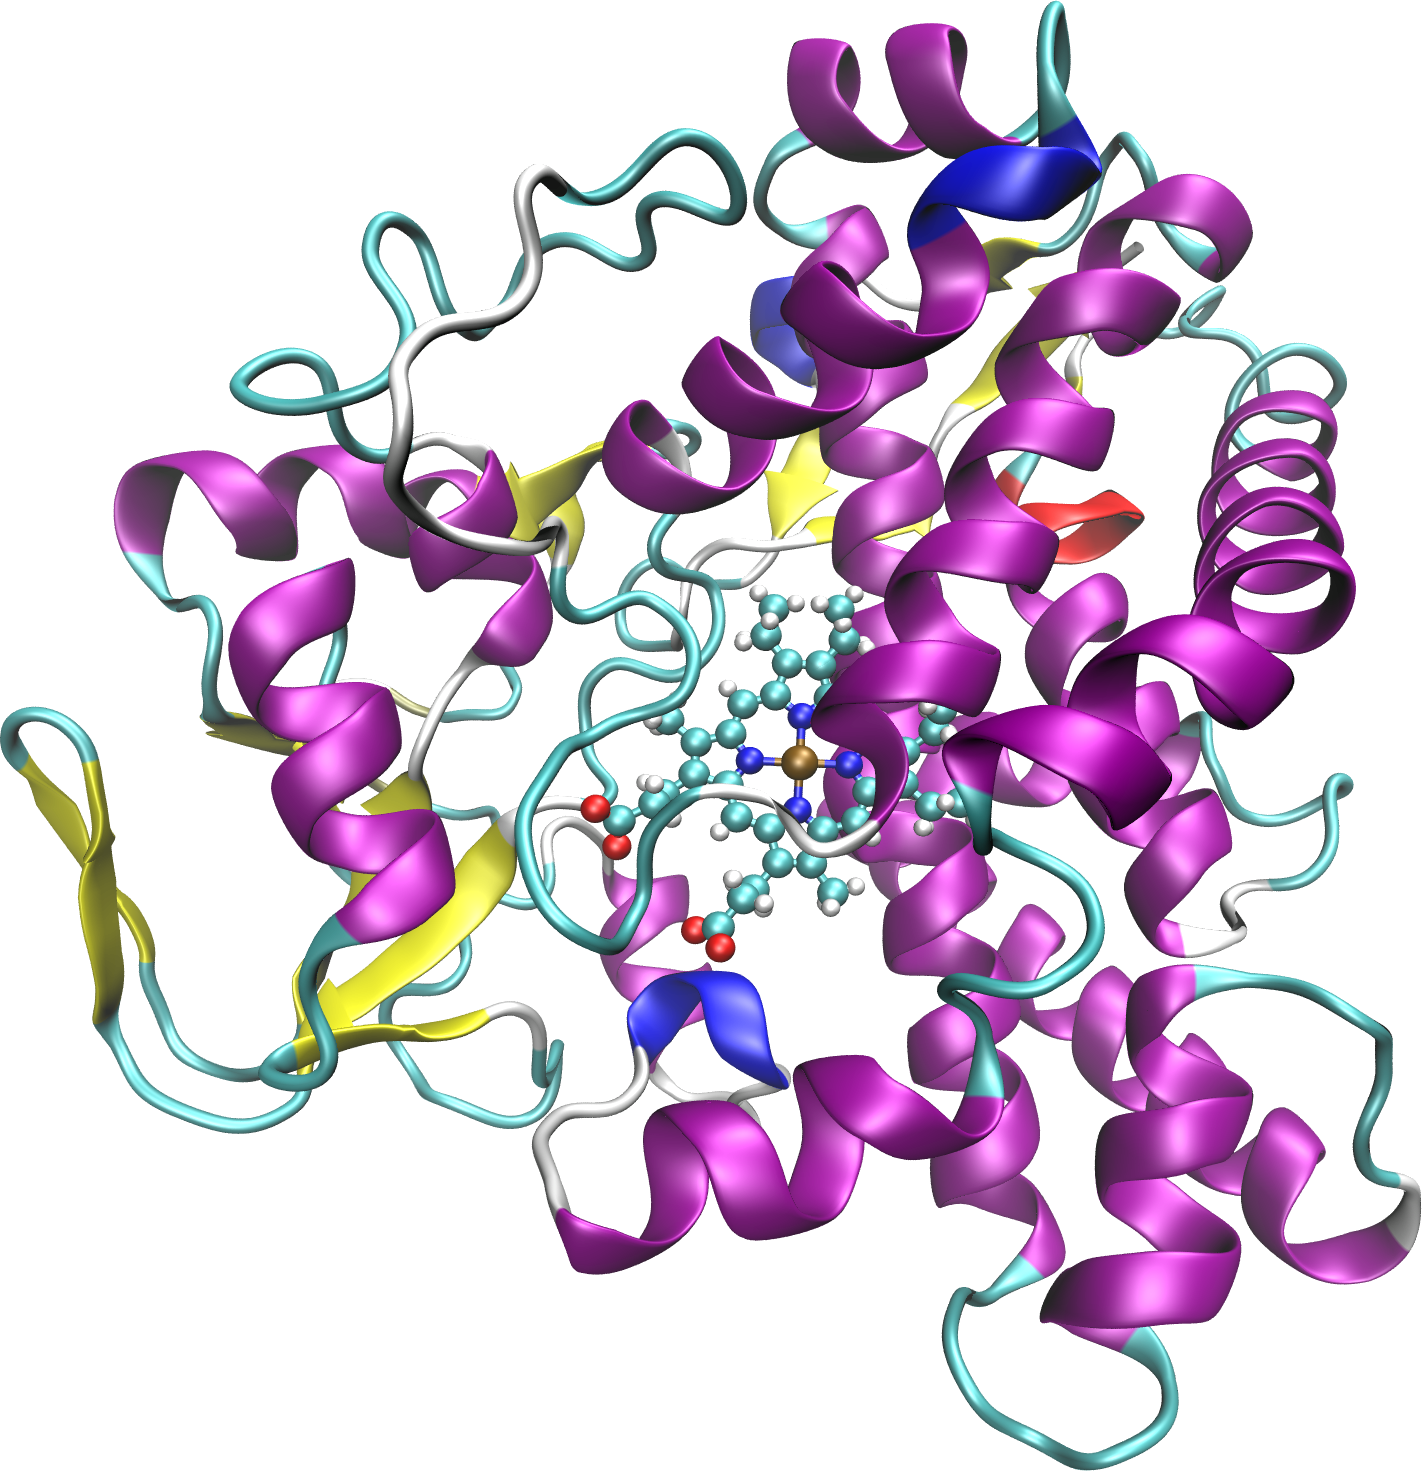
\includegraphics[width=0.5\textwidth]{figures/p450.png}
\caption{
The structure of cytochrome P450, taken from PDBid 1JFB, shown in cartoon representation.
The bonded heme group, shown as ball and stick model, is visible in the center.
}
\label{fig:p450}
\end{figure}


Metropolis Monte-Carlo simulation was originally developed in the 1950's to provide rapid sampling of the solution space of many variable problems \cite{metropolis1953equation,hastings1970monte}.
Monte-Carlo techniques generate a sequence of states from a distribution by proposing a new state based only on the current state 
If the ensemble average is the same as the sequence average, a Monte Carlo Markov chain can be used to estimate ensemble averages, this is known as {\it ergodicicy} \cite{schlick2010molecular}.
Another requirement is {\it detailed balance} that the probability of transition from a state $X_{i}$ to a state $X_{i+1}$ is the same as the probability of the reverse transition, i.e. $X_{i+1}$ to $X_{i}$.
By setting the probability of acceptance to
\begin{equation}
\label{equation:metropolis_acceptance}
P(x \rightarrow x') = min\left(1,e^{-\frac{{\Delta}E}{k_{B}T}}\right)
\end{equation}

these conditions are met.

In molecular mechanics, Metropolis Monte Carlo provides a very efficient means of sampling conformation space and a simple method of estimating the distribution of states.
Modifications on this method, such as annealing, where the temperature is continuously decreased over the course of the simulation, or umbrella sampling, which attempts to achieve better sampling in cases where a potential energy barrier divides two or more states from each other \cite{torrie1977nonphysical}.
While Monte Carlo sampling techniques are very fast to provide new states, the majority of these states reflect higher energy conformations.
Since it is of practical biological interest, Monte Carlo minimization has been developed to increase the rate at which minima are sampled \cite{li1987monte}.


\chapter{Cross Docking}
\label{chapter:cross_docking}
\section{Cross Docking}
\label{section:cross_docking}
\subsection{Cross Docking}
\label{subsection:cross_docking}
\cite{jacobson2004hierarchical}

\chapter{Computational Mutation Scanning}
\label{chapter:mutations}
\section{Computational Mutation Scanning}
\label{section:mutations}
\subsection{Computational Mutation Scanning}
\label{subsection:mutations}
\cite{jacobson2004hierarchical}

\chapter{Hash-Based Implicit Solvent}
\label{chapter:cell_solvent}
\section{Hash-Based Implicit Solvent}
\label{section:cell_solvent}
\subsection{Hash-Based Implicit Solvent}
\label{subsection:cell_solvent}
\cite{jacobson2004hierarchical}


%\part{Title for the first part}
%\label{sec:corpus}
%\input{sample-part}
%\part{Title for the second part}
%\label{sec:corpus}
%\input{sample-part}
%\part{Conclusions}
%\label{sec:conclusions}
%\chapter{Conclusions}

The general conclusions go here.
The general conclusions go here.
The general conclusions go here.
The general conclusions go here.
The general conclusions go here.
The general conclusions go here.
The general conclusions go here.
The general conclusions go here.
The general conclusions go here.
The general conclusions go here.
The general conclusions go here.
The general conclusions go here.
The general conclusions go here.
The general conclusions go here.
The general conclusions go here.
The general conclusions go here.
The general conclusions go here.
The general conclusions go here.
The general conclusions go here.
The general conclusions go here.
The general conclusions go here.


%%% Appendices
%\part{Appendices}
%\appendix
%\input{sample-appendix}
%\input{sample-appendix}

%%% Bibliography
\part{Bibliography}
\addcontentsline{toc}{chapter}{Bibliography}
\bibliography{refs}
\bibliographystyle{named} 

\end{document}
